\documentclass[twocolumn,11pt]{article}

\usepackage[margin=1in]{geometry}
\usepackage{caption}
\usepackage{graphicx}

\title{Journey: A Study of Scalabilty of Memory Management in Linux}
\author{Mark Mansi, Suhas Pai, Hasnain Ali Pirzada\\\texttt{\{markm, spai, hp\}@cs.wisc.edu}}
\date{}

\begin{document}

\maketitle

\begin{abstract}
    \small 

Much research is currently being done to study how non-volatile and large
memory systems would change system design.  We see the need for a lightweight
tool to study such systems at scale with real workloads.  The first step
towards building such a tool is to study the scalability of existing memory
management systems.  We find that in most cases, Linux kernel memory management
scales well with large amounts of physical memory. However, workloads that
allocated many virtual memory areas can accumulate significant memory and
computational overhead due to kernel metadata.     Furthermore, in certain
situations, transparent hugepages can nullify the benefits from better TLB
reaches by inducing memory pressure earlier, even for workloads that would
otherwise not experience it.  Finally, we see that the 99.99-th percentile of
disk latency during swapping can account for over 70\% of runtime for the
workloads we tested.

\end{abstract}

\section{Introduction}

Recent advances in memory technologies are making it possible for machines with
large amounts of memory to become commonplace.
These technology advances can
enable systems with terabytes of memory in the not very distant future. For
example, non-volatile memory technologies, which have denser physical
structures than traditional DRAM are making such large memories available and
more accessible \cite{xpoint}.

Much research is currently being done to study how non-volatile and large
memory systems would change system design. HP has been working on a system
which it calls ``The Machine'', in which hundreds of cores have access to a
multi-petabyte shared memory pool \cite{hp_machine}. Intel and
Micron have announced their 3D Xpoint non-volatile memory technology, making
dense, fast, persistent memory comercially available \cite{xpoint}.

However, studies of large-memory systems are often forced to use simulation or
emulation to evaluate solutions because most researchers do not have access to
these sorts of systems for experimentation \cite{quartz}. This often
forces researchers to simplify models, incurring inaccuracy, or to use smaller
benchmarks, which are less realistic. We note that there was a similar problem
when large storage systems first became available \cite{david, exalt}.

Currently, there are few good tools available to systems researchers for
understanding how systems interact with large memories. An important first step
towards building such a tool is to identify bottlenecks in managing large
memories that make a tool difficult to develop. 

In particular, we look at the case of a single process using a large amount of
memory in a current Linux system. We run experiments to identify the scalability
of the Linux memory management system across multiple dimensions. First, we
measure the overhead of \texttt{vm\_area\_struct}, a common bookkeeping data
structure in the Linux kernel. Then, we measure the memory and processing
overheads of swapping. From these data, we extrapolate to systems running with
more memory; many of the behaviors we identify would be aggravated by having or
using more memory.

While these experiments are not comprehensive, we believe they can offer
insights that are useful both for building a research tool and for building
systems. Also, we focus on large memory systems in general, rather than
persistent memory system in particular.


\section{Background}

In our methodology, we run several experiments to measure the scalability of
the Linux memory management system. Each experiment is designed to probe a
different aspect of the system. This section gives some background knowledge
necessary to understanding the experiments.

\subsection{Virtual Memory Areas}

A process may use the \texttt{mmap} system call to request that the kernel
allocate part of its virtual address space.
The Linux kernel keeps track of which portions of a process's address space
have been allocated using the \texttt{vm\_area\_struct} data structure. Because
processes may map a number of regions, including shared objects, stack, heap,
text, and anonymous regions, the scalability of this structure is critical to
Linux's performance.

When a process maps a region, a \texttt{vm\_area\_struct} is created, but no
memory is allocated. When a process first touches a page, a page fault occurs
and the processor traps to a page fault handler, which allocates memory and
sets up a page table entry for a valid access. This is called demand paging.

For demand paging to work efficiently, the correct \texttt{vm\_area\_struct}
needs to be efficient to find. Linux caches the most recently used region and
organizes all regions into a red-black tree for fast lookup.  Moreover,
adjacent regions with similar permissions and properties are merged in an
effort to keep bookkeeping costs low.

In our first set of experiments, we measure the memory overhead and latency of
the Linux Memory Management system's use of \texttt{vm\_area\_struct}, which
represents a region of a process's virtual address space. All the physical
pages in the system are managed using the \texttt{struct page} descriptors in
the kernel.  We do not measure the overhead of \texttt{struct page} because it
is known that there is one struct for each physical page. We do not measure the
overhead of page tables because this can be calculated from the size of the
virtual memory space used by the process.  

When a program makes a memory
management system call such as \texttt{mmap}, \texttt{mremap}, \texttt{munmap},
\texttt{mprotect}, \texttt{mlock}, or \texttt{madvise}, the kernel is creating,
changing, or removing \texttt{vm\_area\_struct}s; thus, measuring the
scalability of Linux memory management requires measuring the overhead of these
structs.

\subsection{Swapping}

Under memory pressure, the kernel may free some pages for use by writing some
pages to disk. Memory mapped files are written back to their backing files,
but anonymous memory is written to portion of the disk called swap space. We
focus on anonymous memory in our experiments.

Before swapping a page out to disk, the kernel must reserve a slot for the page
in the swap space, unmap it from the process's address space by removing its
page table entries and flushing the TLB, and record which swap slot corresponds
to the page.

On Linux, the system may have multiple swap spaces in the form of a swap disk
partition or of swap files on a filesystem. Both have a similar format on disk,
in which the space is broken into a number of swap slots large enough for one
page. For each of these swap spaces, the kernel keeps a swap map, which records
the usage of each swap slot so that it can find and allocate them quickly.

Unmapping a page from a process's address space involves simply marking its page
table entry ``Not Present''. Rather than using a separate data structure, Linux
uses the unused page table entry to record information about which swap space
and slot is used to swap out the page.

On systems with transparent hugepages enabled, huge pages are not swapped out in
one piece.  They are broken down to their component small pages, which are then
swapped to disk via the normal mechanisms. This is done to simplify the swapping
logic in the kernel, but results in additional overheads
\cite{corbet_transparent}.

\subsection{Page Frame Reclamation}

To determine which pages to swap out, Linux uses the Page Frame Reclamation
subsystem. Choosing which pages to swap out is important because if the system
swaps out pages that are about to be used, thrashing may be induced, in which
the system wastes lots of time swapping out a page just swap it back in.

The Linux Page Frame Reclamation Algorithm (PFRA) attempts to approximate LRU
order. It uses a clock-like algorithm, in which a list of pages is scanned
twice. Roughly speaking, if a page is not used between scans, then it is a
condidate for reclamation.

The PFRA runs primarily as a kernel thread called kswapd. kswapd runs at regular
intervals and sleeps in between. Also, it may be invoked if the system detects
that memory has gone below a threshold. kswapd will continue to run until enough
pages are freed to bring the free memory pool above some threashold. Then,
kswapd goes back to sleep \cite{utlk}.  One concern with systems that have a large memory
usage is that kswapd may expend significant CPU time scanning through hundreds
of thousands of pages.

\section{Methodology}

We conduct a series of experiments to measure the scalability of various parts
of the Linux memory management system.  First, we measure the scalability of
Linux's \texttt{vm\_area\_struct}. Then, we measure the scalability of Linux's
swapping mechanisms.

\begin{figure}[t]
\centering
\begin{tabular}{|l|p{5cm}|} \hline
OS & Ubuntu 16.04.2 \\ \hline
Kernel & Linux 4.4.0-70 \\ \hline
CPU & Intel Xeon E5645, 2.40 GHz, 6 cores/12 threads, 32kB L1-D, 32kB L1-I,
    256kB L2, 12MB L3 \\ \hline
Memory & 16GB, 1066MHz \\ \hline
Storage & 500GB HDD, 7200RPM \\
\hline
\end{tabular}
\caption{Specifications of our test machine.  \label{fig:specs}}
\end{figure}

The specifications of the machine we used to run our experiments are listed in
Figure \ref{fig:specs}. We disabled Intel SpeedStep and TurboBoost and ensure
that the processor frequency stays constant. All experiments are pinned to the
same core on our machine. 

We run several different microbenchmarks, each of which has a different memory
allocation pattern. These benchmarks are designed to stress the memory
management system in different ways, rather than simulate real workloads. 
Each run is executed in isolation, without any additional processes
running beyond services that start when the system is booted and a single ssh
session. We are careful to avoid opening extra ssh sessions, running screen or
tmux, or executing extra commands while a benchmark is running since these may
impact memory usage and, thus, our results.

We measured latency using the \texttt{rdtsc} instruction provided by x86\_64
processors, which gives high resolution cycle-level timestamps. We take a
timestamp before and after each memory management operation in the workload and
take the difference to get latency.

% TODO: should we mention slab allocator?
% (MM) I don't thinks so...
To measure memory usage, we use the procfs's reporting on current memory usage.
Where appropriate, we record the number of active
\texttt{vm\_area\_struct}s in the system. Measuring kernel memory usage and
associating memory usage with a particular process is difficult. Our methodology assumes
that our benchmarks are running in an otherwise idle system and should dominate
increases in memory usage.  We compute total memory usage by the rest of the
system as the total amount of memory less the amount of memory used by the
benchmark. We keep transparent huge pages on throughout our experiments, unless
otherwise specified.

To measure processor usage, we use the procfs's reporting on number of jiffies.
\texttt{/proc/stat} reports the number of jiffies of uptime the system has seen
overall, while \texttt{/proc/[pid]/stat} reports on the specified process.

\subsection{\texttt{vm\_area\_struct} Experiments}
\label{ss_vm_area_struct}

For each workload, we measure the latency and increase in memory usage due to
each operation in the benchmark. Notably, we do not touch the pages that we
allocate, avoiding both a page fault and the allocation of a backing physical page
for the allocated virtual pages. This allows us to measure just the overhead of
memory management, as opposed to physical page allocation, swapping, page
faults, or other overheads.  Each workload contains $2^{20}$ memory management
operations.

Each benchmark was run 5 times and the results aggregated as described below. We
reboot the machine when switching to a different benchmark, but keep the machine
running continually during the runs of the same benchmark. 

Assume the memory usage of the rest of the system is $R$. We denote $R_i$ as the
$i$-th measurement of $R$ during a run ($i = 0, 1, ..., 2^{20}$). System memory
usage is known to jitter in Linux \cite{jitter}. To adjust for this jitter, we
define $\Delta_i = R_i - R_0$. For each operation, we take the median value of
$\Delta_i$ across the 5 runs to reduce jitter further.  This is the value
graphed in the figures in the following section. $\Delta_i$ represents the
increase in memory usage due to memory management overheads caused by running
$i$ memory management operations.

The workloads we measure are

\begin{itemize} \item \textit{Control}. This workload is only run for the memory
overhead experiments. It simply prints the $\Delta_i$ for each $i$. It's graph
is a straight line with positive slope. This memory usage results from the
buffer containing stdout, where our readings are being printed. All of our
experiments have the same stdout overhead, so this benchmark serves a baseline
for comparison.

\item \textit{Continuous} (\texttt{cont} for short). This workload allocates $2^{20}$
adjacent 16KB blocks.

\item \textit{Strided}. This workload allocates $2^{20}$ untouching 16KB regions
in order of increasing memory address.

\item \textit{Random}. This workload randomly allocates the pages in a
$2^{20}$ page region.

\item \textit{Fragmented} (\texttt{frag} for short). This workload first allocates
    $2^{21}$ contiguous 4KB blocks. Then, it resizes every other block to 16KB.
        The resizing operation, rather than the initial allocation, is measured.
        By resizing every other block, rather than every block, the number of
        worst-case operations is maximized because the kernel must move each
        resized block.
\end{itemize}

\subsection{Swapping Memory Overhead}
\label{swapping_memory_overhead}

These experiments are designed to measure the minimum amount of memory needed
by the swapping subsystem itself.

A single process allocates 18GB of virtual memory space. It then proceeds to
write one byte of each 4KB page in the region, leading to the actual allocation
of physical memory. Notice that 18GB exceeds the 16GB of physical memory in the
test machine, causing Linux to start paging after physical memory is exhausted.
Also, notice that the Linux kernel will reserve some memory for its own
operation.

We run this experiment with both a continuous access pattern and a random access
pattern. The continuous access pattern simply touches adjacent pages in order of
increasing address. The random access pattern chooses a random address. Both
patterns touch the same number of addresses.

After each page of virtual memory is touched, the resident set size (RSS) is
recorded. The RSS is the
amount of physical memory Linux has allocated to the process. The
values of RSS are stored in an mlocked array and written to a file after the
benchmark completes. This prevents the writing of the results from interacting
with paging in the kernel page cache. These RSS values are graphed in our
results section.

Moreover, we measure the latency of each memory store operation to see the
impact of swapping and virtual memory usage on memory access times.

We repeat this with 32GB of swap space and 128GB of swap space to see the
impact of swap space size on the amount of memory the kernel reserves for
itself, along with the impact on latency.

\subsection{kswapd}

These experiments are designed to measure the processing overhead of kswapd when
the system is under high memory pressure.

As in the previous set of experiments, a single process allocates 18GB of virtual memory space and writes one byte of
each 4KB page in the region. The same two access patterns are tested as in the
previous set of experiments (continuous and random).

In all these experiments, the system is given 32GB of swap space total. We
repeat each experiment with hugepages enabled and disabled to see the impact of
the transparent hugepage system. The processor usage of kswapd is
recorded for each experiment and reported in the next section.

%A SQL query goes into a bar, walks up to two tables and asks, ``Can I join you?".

\section{Results}

\subsection{\texttt{vm\_area\_struct} Experiments}

\begin{figure}[t]
    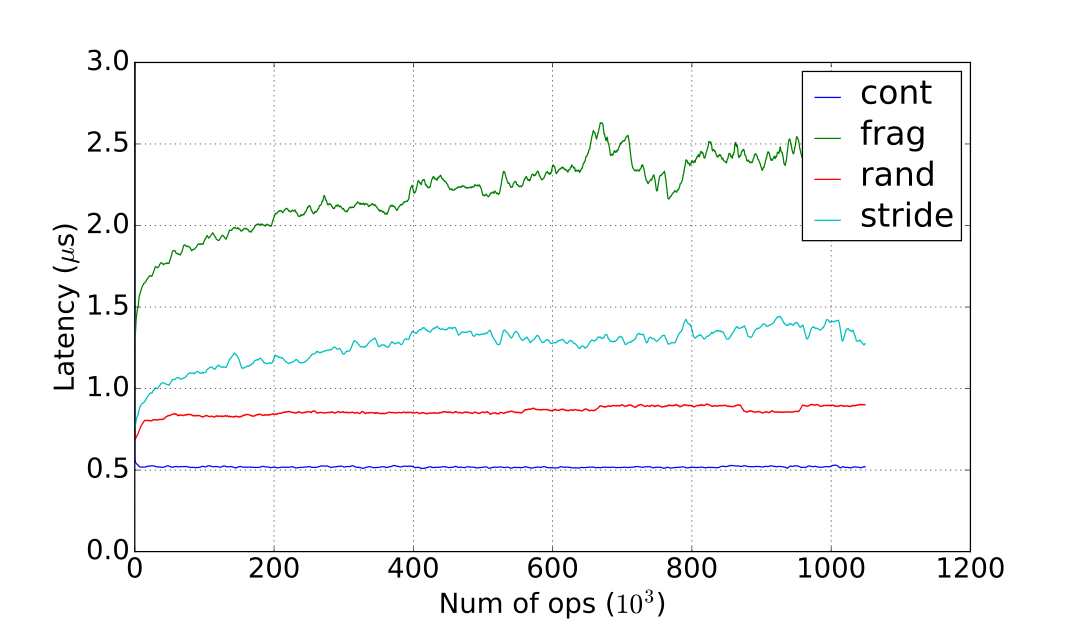
\includegraphics[width=\columnwidth]{figures/mmap_latency}
    \caption{Latency of memory operations. A running average with window of
    width 5000 operations is used to reduce jitter.}
    \label{fig:mmap_latency}
\end{figure}

\subsubsection{Memory}
Figure \ref{fig:mmap_mem_usage} shows the growth in memory usage of the system
for the workloads described in section \ref{ss_vm_area_struct}. 

The
\texttt{cont} workload coincides with the \texttt{control} workload, as only the
first \texttt{mmap} operation allocates a \texttt{vm\_area\_struct}. The subsequent
operations are subsumed by the initial \texttt{vm\_area\_struct} because the mapped
regions are adjacent, and hence the memory usage does not increase despite the
large number of \texttt{mmap} operations.  

The \texttt{stride} workload allocates a
\texttt{vm\_area\_struct} for each operation due to the separation of
allocations in the virtual address space. As a result, the memory usage
increases significantly as more memory is consumed with each \texttt{mmap} operation.

This is also the case for the \texttt{frag} workload which breaks up a single
\texttt{vm\_area\_struct} for a large area in the virtual address space into
multiple smaller areas, which results in the allocation of a new structure for
every resize operation. 

The \texttt{rand} workload initially creates a new
\texttt{vm\_area\_struct} struct for each \texttt{mmap} operation. Eventually, these
allocations form larger contiguous allocations when two or more regions are
mapped next to each other, resulting in a single \texttt{vm\_area\_struct} being
used for that range. As a result, the memory usage begins to taper off and
even decreases slightly as multiple \texttt{vm\_area\_struct}s are collapsed to
single structures. This is made clear by Figure \ref{fig:vm_area_struct_count}
which shows the growth \texttt{vm\_area\_struct} counts for each workload.

~\\ \textbf{Insights}

The memory overhead of \texttt{vm\_area\_struct}s increases linearly with the
number of mapped regions when these regions are separated by unused memory
addresses. When a workload maps a large number of regions, this overhead can be
on the order of hundreds of megabytes to gigabytes for large memory systems.  To
reduce this overhead, it is crucial that regions with similar access permissions
are placed adjacently in the address space so that they can be identified by a
single structure. It is important for large applications such as object-oriented
databases that map a large number of regions to be aware of these overheads and mitigate them \cite{utlk}.

\subsubsection{Time}

Figure \ref{fig:mmap_latency} shows the time taken
per \texttt{mmap} operation as it varies with the total amount of memory allocated
so far by the workload. 

It can be seen that for continuous \texttt{mmap}s the time is not only the
lowest but is also invariant with the total number of \texttt{mmap}s done so
far. There are two reasons for this. 

First, when a continuous \texttt{mmap} happens, the
kernel memory allocator does not need to create a new \texttt{vm\_area\_struct}.
Instead, it uses the existing \texttt{vm\_area\_struct} to account for the
newly allocated space. This obviates the need to use the slab allocator to create
a new struct. 

Second, by caching the
most recently used \texttt{vm\_area\_struct}, the kernel avoids a search in the
red-black tree. In the \texttt{cont} benchmark, this cached struct is always
conveniently used.

For the other workloads, a search through the red-black tree is often needed on
most accesses. This operation takes $O(log n)$ time, where $n$ is the number of
virtual memory areas. The logarithmic behavior is visible in the plots for the
benchmarks in Figure \ref{fig:mmap_latency}.

The \texttt{frag} benchmark takes the most time of any benchmark. When a region of the
address space is being expanded, the kernel is forced to unmap it and map a new
area elsewhere in the address space. This operation needs creation of a new
\texttt{vm\_area\_struct}.  The kernel also must search through the red-black
tree, though it never finds a node which can be expanded to include the new
mapping. Then, an insertion on the tree is needed, possibly including
rebalancing. Moreover, the existing \texttt{ vm\_area\_struct} needs to be
removed from the tree. 

The \texttt{stride} workload is very similar to \texttt{frag} because it will also force the
kernel to always create a new structure and insert it into the tree after
traversing the tree first. However, it does not need to delete an existing
structure, which causes it to be faster than the \texttt{frag} benchmark.

Finally, the \texttt{rand} workload will also search through the red-black tree first,
but there is a reasonably high probability that it will find an existing
mapping adjacent to the desired mapping which can be expanded, obviating the
need to create a new struct and insert it into red-black tree. Therefore, usually
the time taken by \texttt{rand} benchmark is lower than \texttt{stride}.

%When your hammer is C++, everything begins to look like a thumb.

~\\ \textbf{Insights}

Linux's use of \texttt{vm\_area\_struct} tends to be scalable in the general
case. The kernel latency of creating a memory region is lowest when the new
memory is allocated next to an already allocated region. This latency is the
worst in the \texttt{frag} microbenchmark i.e., when an already mapped region
is to be expanded.  We recommend that applications that manage their own memory
and expand memory regions should avoid this pattern.

\begin{figure}[t]
    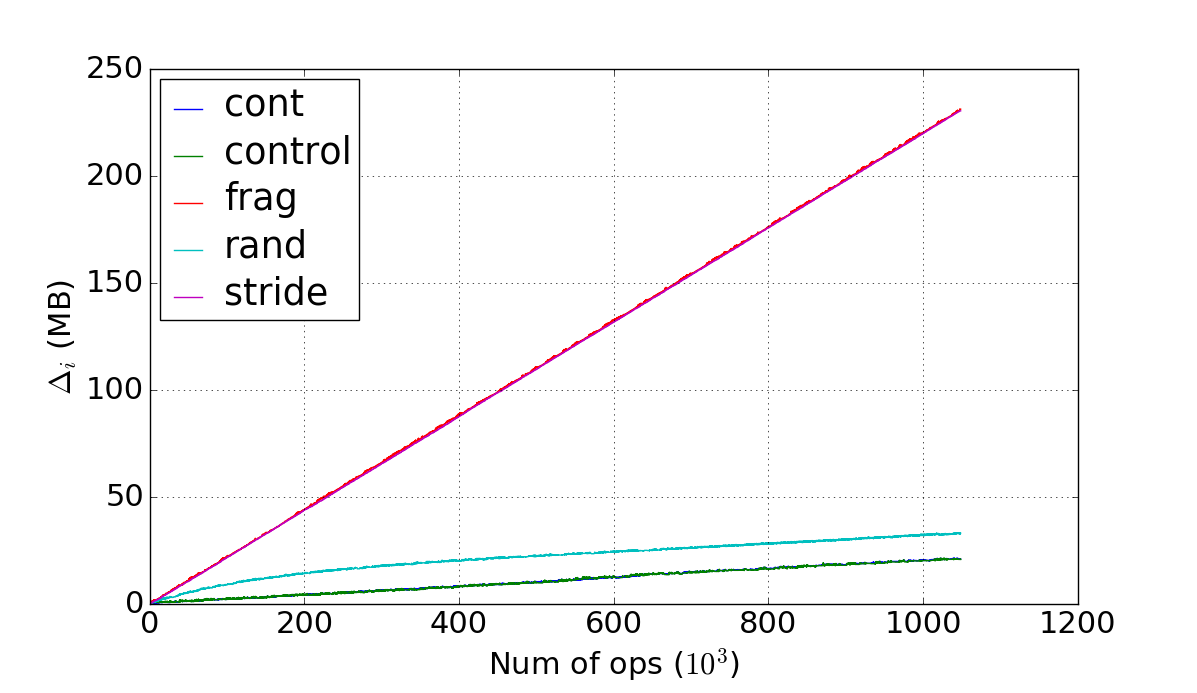
\includegraphics[width=\columnwidth]{figures/mmap_mem_usage}
    \caption{$\Delta_i$ adjusted with \texttt{control} for benchmarks. Note that
    graphs of \texttt{frag} and \texttt{stride} overlap. Also, \texttt{cont} and
    \texttt{control} overlap.}
    \label{fig:mmap_mem_usage}
\end{figure}

\begin{figure}[t]
    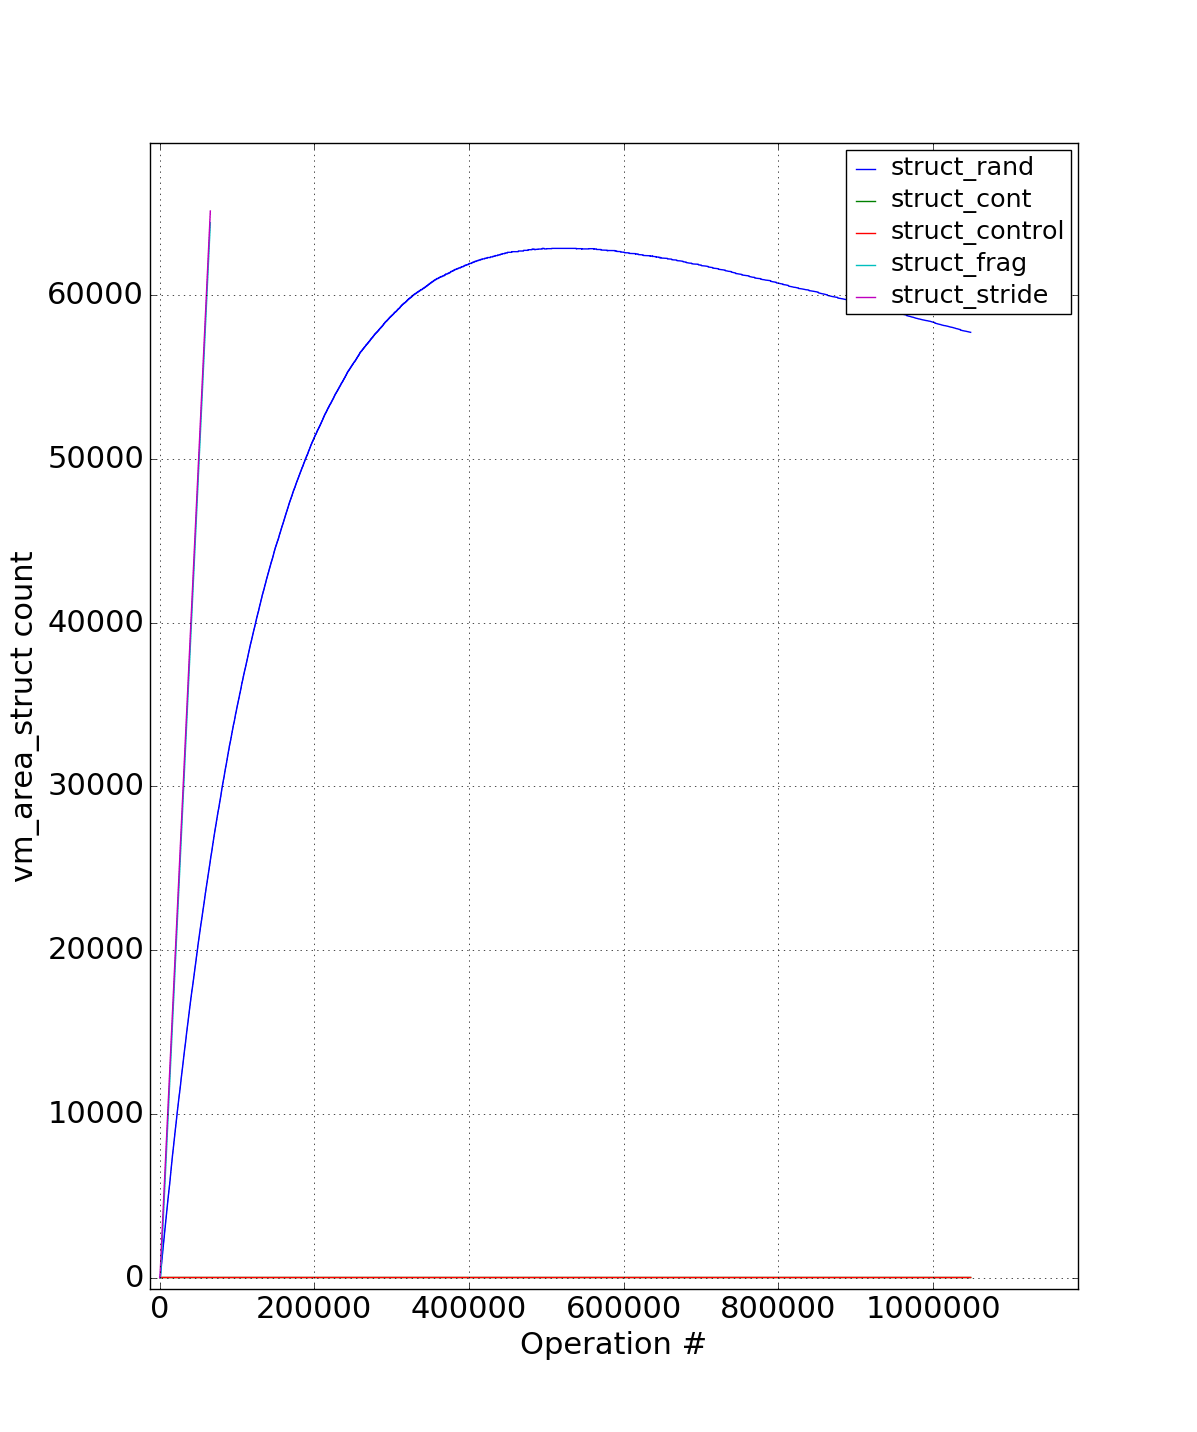
\includegraphics[width=\columnwidth]{figures/vm_area_struct_count}
    \caption{Number of \texttt{vm\_area\_struct}s for benchmarks}
    \label{fig:vm_area_struct_count}
\end{figure}


\subsection{Swapping Experiments}

\subsubsection{Memory}

\begin{figure}[t]
    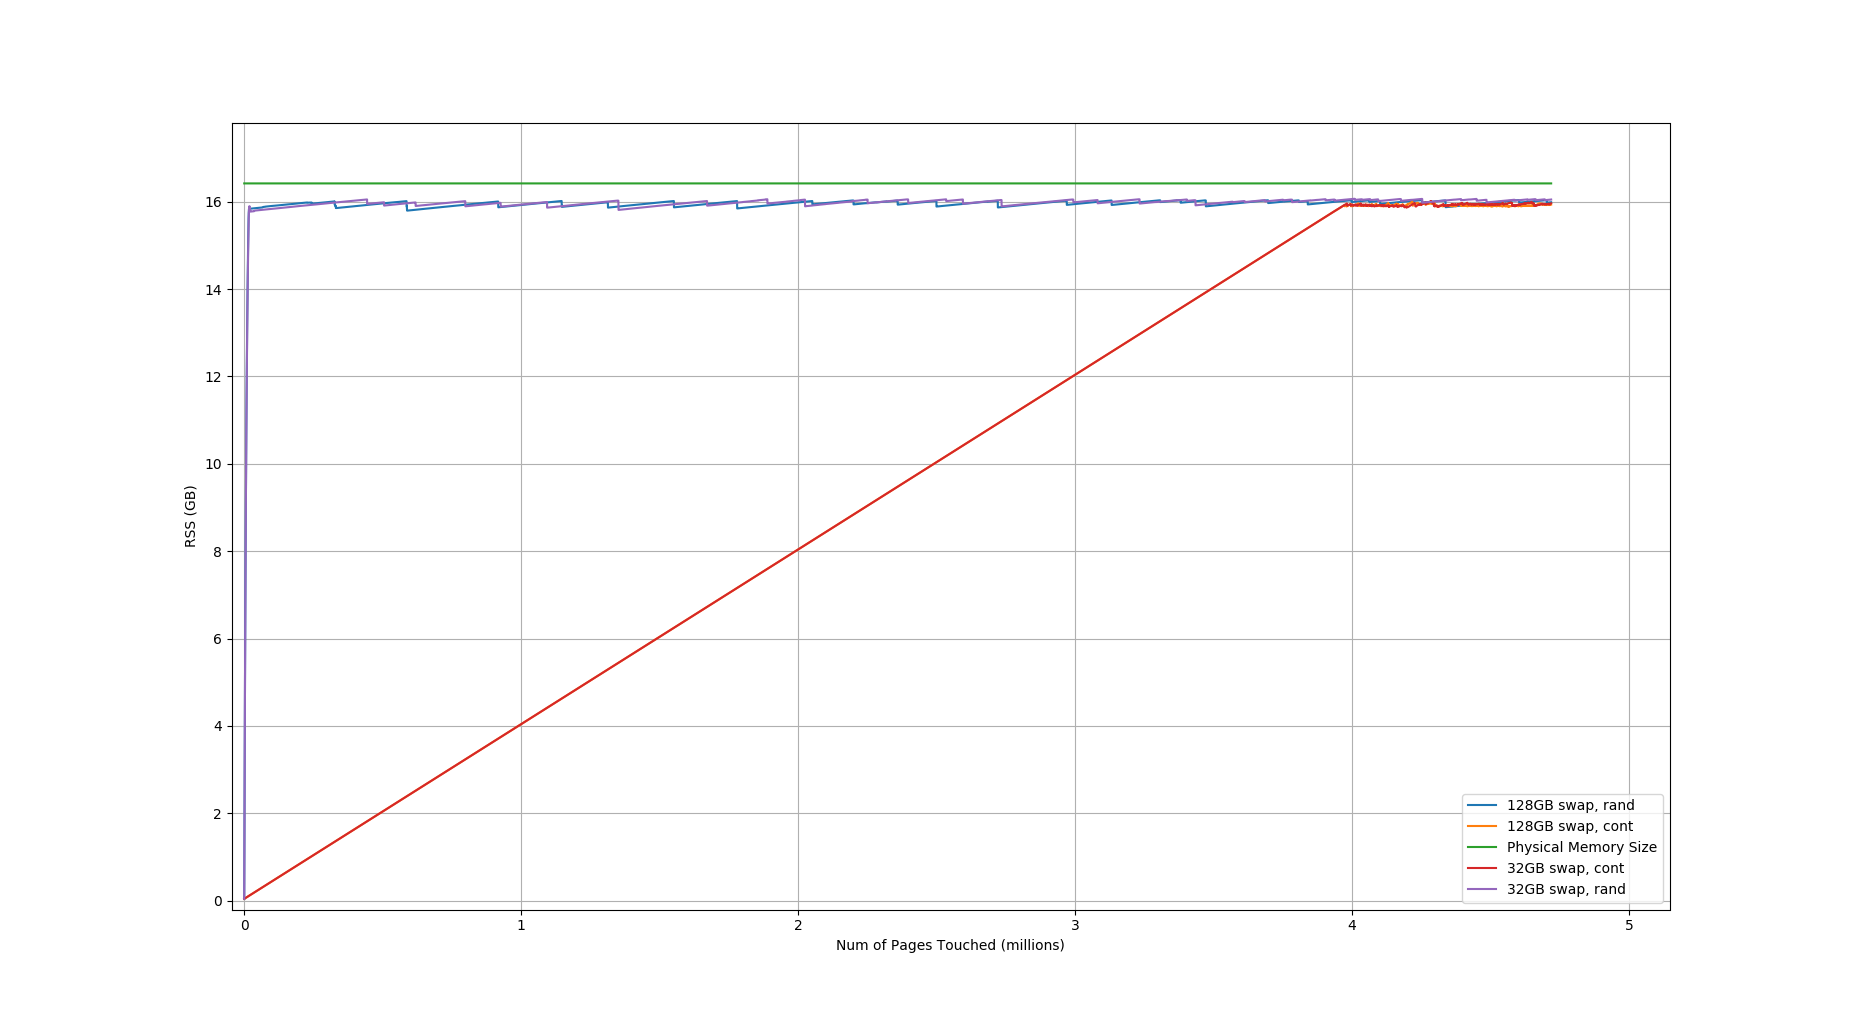
\includegraphics[width=\columnwidth]{figures/swap_rss}
    \caption{RSS while touching pages.  \label{fig:swap_rss}}
\end{figure}

Figure \ref{fig:swap_rss} shows the RSS of each workload for the
experiments described in section \ref{swapping_memory_overhead}. 

The \texttt{cont} workload writes to adjacent 4KB pages in the address space. A huge page
of size 2MB is allocated when a new page is touched initially. Subsequent 4KB
pages that are touched are subpages of the 2MB page allocated initially. As a
result, the memory used by the workload is almost equal to the amount of memory
it has written to. The RSS thus increases linearly until the system begins to
swap when the number of free pages falls below a threshold. 

The \texttt{rand} workload, on the other hand, writes to pages that are likely not
adjacent and likely not subpages of a single huge page. As a result, a huge page
is allocated with almost every write, and system memory is exhausted and begins
swapping very quickly (20,000 operations compared to 4 million with the \texttt{cont} benchmark). Memory made available by kswapd is quickly consumed by
further allocations. Hence, the memory used by the workload continues to stay
close to its peak value. As expected, the behavior is the same irrespective of
the size of the swap file.

% If you put a million monkeys at a million keyboards, one of them will eventually write a Java program. The rest of them will write Perl programs.

~\\ \textbf{Insights} 

Transparent huge pages can consume a large fraction of memory and lead to early
onset of memory pressure for workloads with random access pattners. The overhead of swapping greatly exceeds the
performance benefits provided by huge pages. As a result, the workload
performance can fall drastically in such cases. It might be advisable to
disable transparent huge pages for such applications. The kernel can also be
cautious and limit the allocation of huge pages to processes in order to
prevent early onset of memory pressure.

\subsubsection{Time}

\begin{figure}[t]
    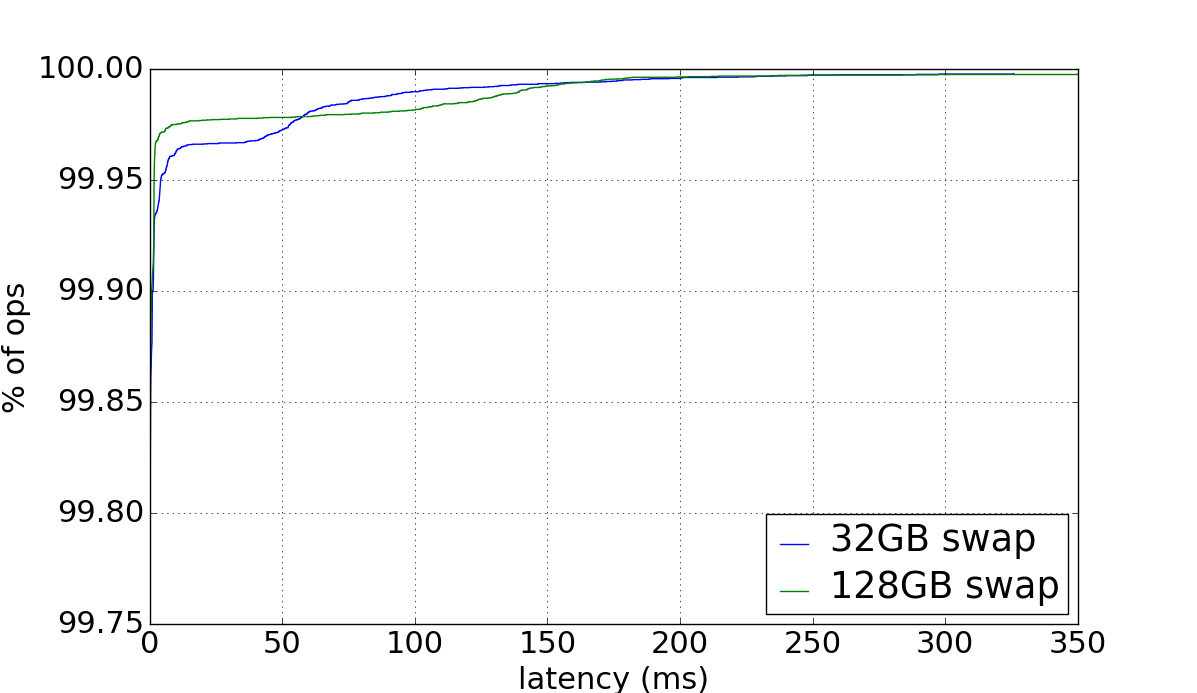
\includegraphics[width=\columnwidth]{figures/swap_touch_time_cont_cdf}
    \caption{CDF of time to touch a page while swapping for \texttt{cont}
    benchmark. Notice that the y-axis scale is from 99.75\% to 100\%.
    \label{fig:swap_time_cont_cdf}}
\end{figure}

\begin{figure}[t]
    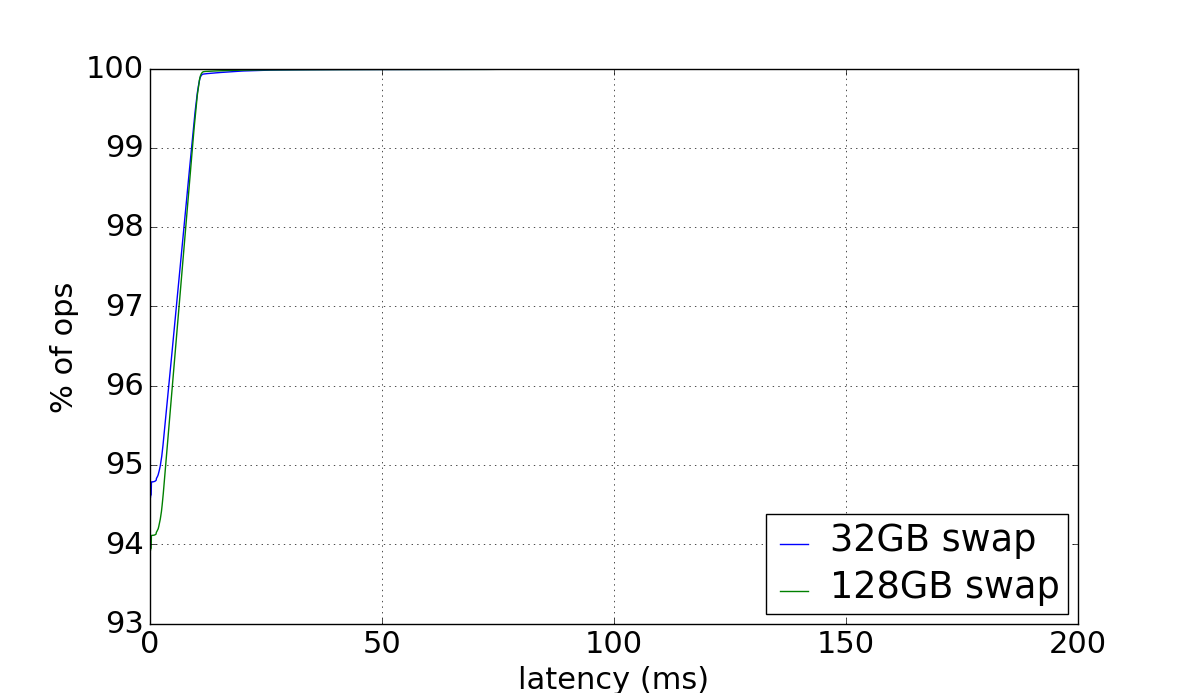
\includegraphics[width=\columnwidth]{figures/swap_touch_time_rand_cdf}
    \caption{CDF of time to touch a page while swapping for \texttt{rand} benchmark.
    Notice that the y-axis scale is from 93\% to 100\%.\label{fig:swap_time_rand_cdf}}
\end{figure}

%\begin{figure}[t]
%    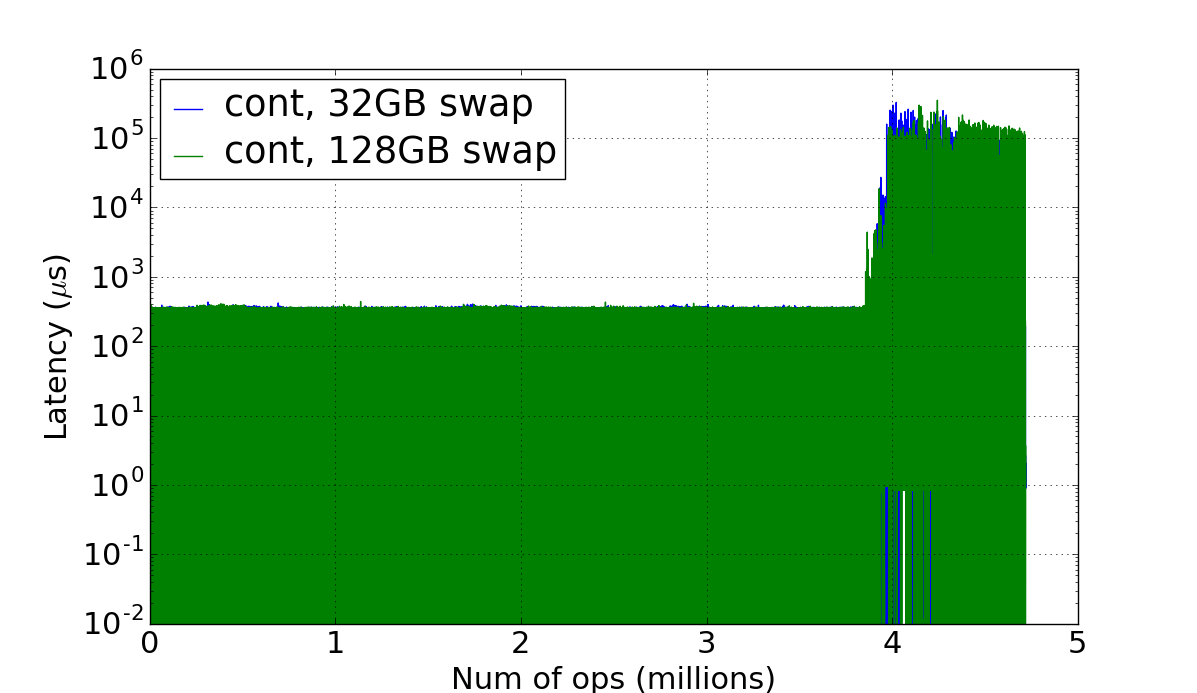
\includegraphics[width=\columnwidth]{figures/swap_time_cont}
%    \caption{Time to touch a page while swapping for \texttt{cont} benchmark.
%    Notice that the y-scale is logarithmic.\label{fig:swap_time_cont}}
%\end{figure}
%
%\begin{figure}[t]
%    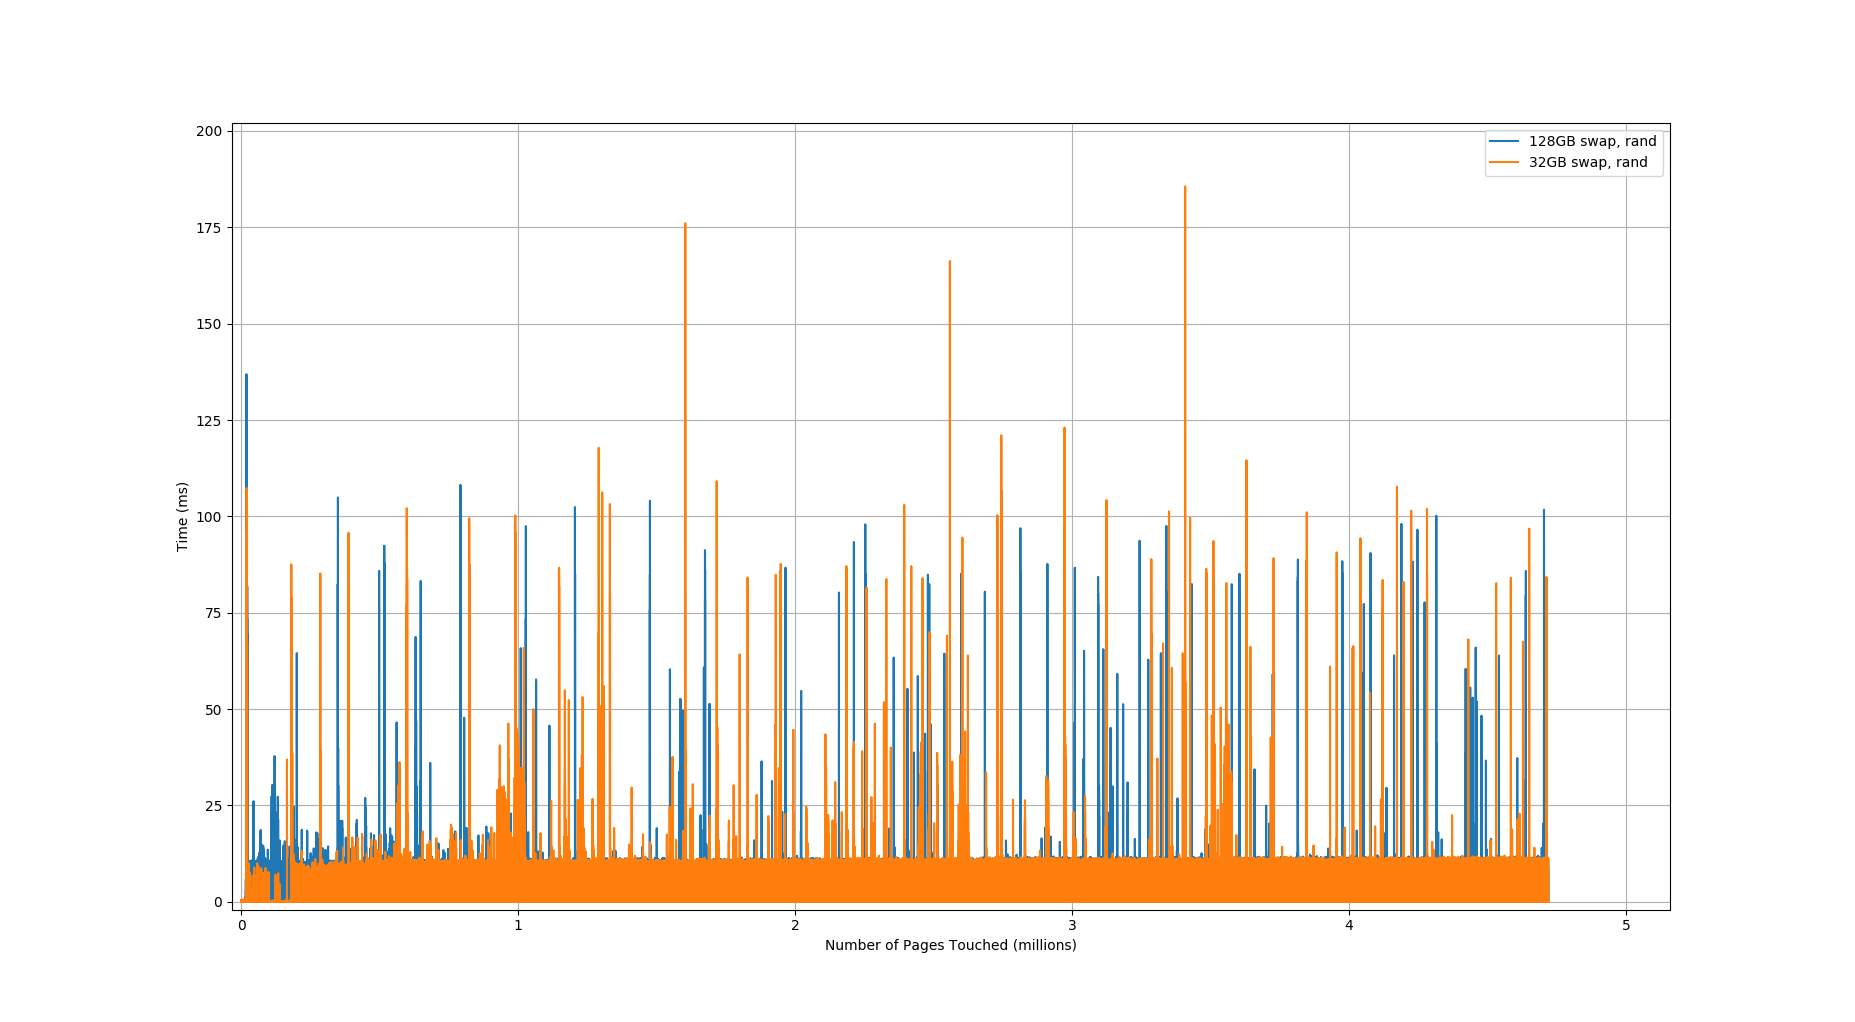
\includegraphics[width=\columnwidth]{figures/swap_time_rand}
%    \caption{Time to touch a page while swapping for \texttt{rand}
%    benchmark.\label{fig:swap_time_rand}}
%\end{figure}

\begin{figure}[t]
    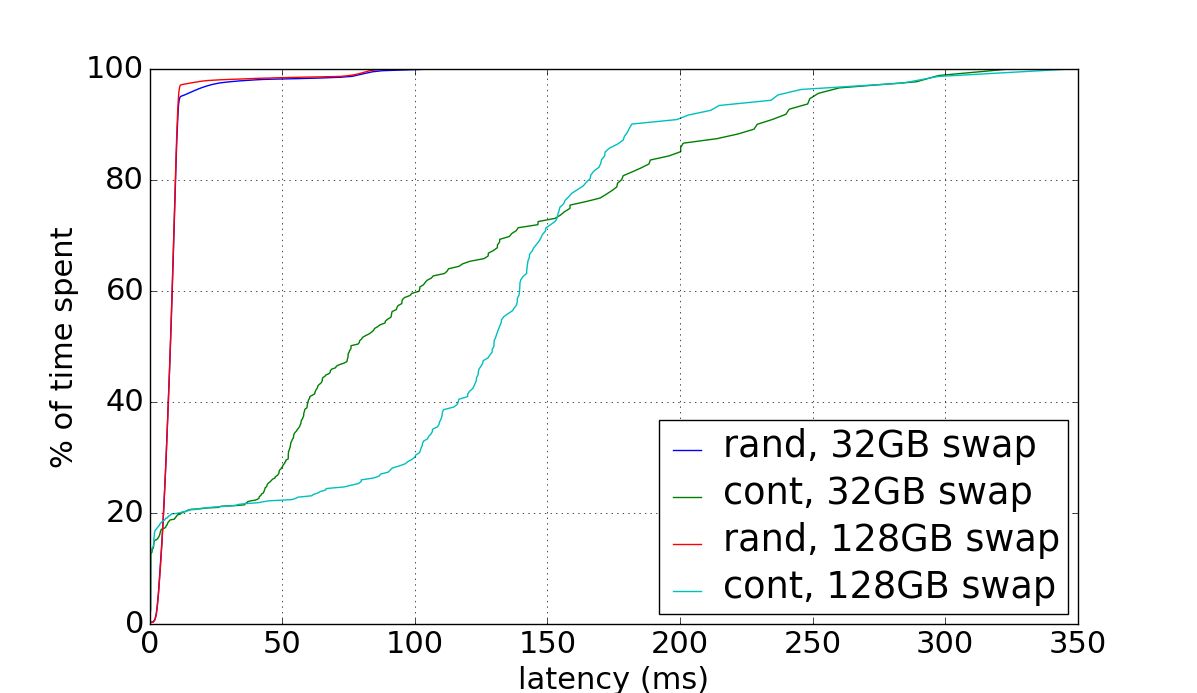
\includegraphics[width=\columnwidth]{figures/swap_time_cdf}
    \caption{CDF of amount of time spent on operations with a given
    latency.\label{fig:swap_time_cdf}}
\end{figure}

This experiment is designed to measure the impact of swapping on memory
operation latency.

The overall behavior is as expected. In the \texttt{rand} benchmark, as before, all
memory is exhausted quickly, and the benchmark induces swapping soon after the
benchmark begins. Many memory accesses thus take milliseconds to complete
because they require paging in or out, which is slow due to disk access.
Even so, the majority of benchmark run time comes from a minority of accesses.
Figure \ref{fig:swap_time_rand_cdf} shows that as much as 95\% of memory
accesses occur on the micro-second scale. Of the remaining 5\%, almost all
accesses complete in less than 20ms. Moreover, notice that the size of the
swap file makes very little difference in this workload because the disk has to
do random seeks regardless of swap file size.

The \texttt{cont} benchmark has more surprising results.
The system only begins to
swap after about 4M operations, as before. Unlike the \texttt{rand} benchmark, we see a
number of operations that take hundreds of milliseconds. Figure
\ref{fig:swap_time_cont_cdf} shows that these only form a fraction of a percent
of all accesses done after swapping starts. However, Figure
\ref{fig:swap_time_cdf} shows that these few accesses form a majority of run
time; they impact performance significantly.

We also find that in the \texttt{cont} benchmark, a larger swap file actually has
slightly more of these slow memory accesses. We believe this has to do with the
fact that the large swap file has less disk locality, and so causes more disk
seeks when paging out. Figure \ref{fig:swap_time_cdf} shows that with a larger
swap file, the \texttt{cont} benchmark has a significantly higher number of
high-latency accesses as compared with the smaller swap file.

The latency of our disk leads us to expect that swapping out pages should take
roughly 4ms. However, we see that in both benchmarks, there are operations that
take dozens or hundreds of milliseconds. We used the \texttt{ftrace} kernel
profiling mechanism in Linux to find out what causes some operations to be
extremely slow.

Surprisingly, the majority of this latency comes from kswapd itself. kswapd goes
through phases of moving pages to the inactive list and reclaiming pages from
the inactive list. This repeated until the amount of free memory increases
beyond a threshold. kswapd does not do any particularly expensive operations
beyond disk I/O. Rather, it executes a bunch of cheaper operations (e.g.
checking if a page was referenced or freeing a page) millions of times in deeply
nested loops. Meanwhile, the workload continues to use up any memory reclaimed
by kswapd. Whenever kswapd is invoked by the page fault handler, it blocks the
faulting process until enough pages are reclaimed.  Moreover, in some cases,
during the \texttt{cont} workload kswapd chooses pages to reclaim much faster
than they can be written to disk.

~\\ \textbf{Insights} 

While large swap files allow greater amount of memory overcommitment, they can
also reduce the degree of disk locality. Thus, large swap files should be
created with disk locality in mind. Some Linux distributions, such as
Ubuntu, have switched to using swap files rather than swap partitions by default
\cite{swap_ubuntu}. Our results suggest that for some workloads this may have a
negative impact on performance if the swap file ends up in non-continuous disk
locations.

% Mark was telling Suhas a TCP joke the other day. He had to keep repeating it slower
% and slower until Suhas got it.

Also, looking at tail latencies is important because they can have a large
impact on overall run time. As our results show, even very uncommon high-latency
operations may have a significant impact on performance.

Our results also show that in some cases, kswapd induces more overhead to choose
a good page to reclaim than would be accrued by choosing the wrong page to
reclaim. Most of this overhead seems to be due to the poor asymptotic complexity
of PFRA. Moreover, the swapping subsystem should be aware of disk bandwidth and
latency, since they fundamentally limits how much memory can be reclaimed per
unit time.

Systems with larger memory may conceivably support more memory overcommitment,
so improving the performance of swapping may be highly relavent moving forward.
Additionally, if a system has orders of magnitude more pages, kswapd may spend
significantly more time scanning the active and inactive lists.

%I would tell you a UDP joke, but you might not get it. Well, even if you got it, you
% wouldn't acknowledge it.

\subsection{kswapd}

Figure (TODO) shows the total number of jiffies spent running kswapd as the
number of operations performed increases. Notice that one jiffy corresponds to
10ms of runtime.

First, we find that number of jiffies is a very imperfect measure of CPU runtime
for kernel threads because it often misses executions of PFRA in the context of
page faulting processes. Due to time constraints, we were not able to rerun our
experiments using a better metric. However, these results do complement our
findings from the previous set of experiments by showing the amount of time
kswapd runs in its own context.

kswapd does not take up a significant percentage of foreground runtime compared
with the applcation. The behavior of kswapd depends heavily on the workload and
on whether transparent hugepages are enabled. Not surprisingly, workloads that
do not exhibit memory pressure do not incur kswapd overhead, as shown by the
\texttt{rand} benchmark with hugepages off.

As expected, the \texttt{rand} benchmark with hugepages on incurs the highest
total overhead since it begins swapping very early. For this benchmark we
observe an overhead of roughly 0.0002 jiffies per page memory touched after
swapping begins. Also, kswapd runs for longer periods of time with longer
intervals of sleep in between. This is most likely because the benchmark has
some probability of retouching a page, so free memory is used more slowly, but
kswapd also has to do more work to find pages that are inactive.

In contrast, the \texttt{cont} benchmark with hugepages disabled uses
computational time at roughly 0.0572 jiffies per page of memory touched.
kswapd runs more frequently and for shorter periods of time because new pages
are touched very quickly, requiring faster reclamation, but because all pages
are only touched once, kswapd has to do very little work to choose pages to
reclaim.

Notice also that the \texttt{cont} benchmark with hugepages enabled spends
surprisingly little time in kswapd. We suspect that kswapd runs once and choose
a large number of pages to swap out. Subsequently, both the workload and kswapd
wait for I/O. This seems consistent with our previous results, in which some
operations take on the order of seconds to complete, but we have not yet
verified it.

~\\ \textbf{Insights} 

The swapping system in Linux has complicated interactions with workloads and
transparent hugepages. It is not obvious how to optimize a workload for better
swapping behavior. Moreover, we see that under memory pressure, kswapd tends to
run more often during page faults than in its own context.

\section{Related Work}

%Initially, we had intended to build a tool for studying large memory systems.
%We found that the first step in doing so is studying the scalability of current
%memory management systems themselves. Thus, our related work section, while
%still relevant to our overall goal, is more directed at the second step of
%building the tool.

The emergence of new technology has in the past often required operating systems
to change. A study of recent changes to memory management in Linux has found that there
has been a lot of focus on improving the scalability of data structures used in
the Linux memory manager \cite{huang2016evolutionary}. Since systems with
persistent memory are expected to have large amounts of memory, there have been
efforts to reduce the overheads of \texttt{struct page}. This is because these
structures can consume several gigabytes of memory for systems with terabytes
of persistent memory \cite{corbet_persistent_progress}. These structures need
to be stored in volatile memory not only because they need to be accessed
quickly for performance reasons, but also to avoid wearing out of persistent
memory due to frequent writes to this data structure. Patches proposed to the
Linux kernel have proposed getting rid of the \texttt{struct page} altogether.

Traditionally, OS researchers and developers would benchmark and test such
solutions in new environments to demonstrate their efficacy before using them in
real systems. However, researchers do not always have access to new technology
for practical reasons; for example, large memory systems are still too expensive
for most research budgets. This is not the first time that researchers have been
forced to study systems in environments they do not have access to. This section
examines past approaches to studying these systems and motivates the need for
our work.

The emergence of the internet required businesses to buy expensive machines to
keep up with demand for their services, but systems researchers did not have
access to these machines. Alameldeen et al. describe how they simulate a
multi-million dollar server using a \$2000 workstation. To do this, they go
through several rounds of scaling down, optimizing, changing, and tuning both
the benchmarks and systems they test. For example, they scale down a workload
to fit in the 1GB memory of the machine they use and increase the number of
threads to improve parallelism \cite{2kmachine}. This methodology may be
accurate, but it requires modifying the benchmarks, which is error prone and
time consuming.  Ideally, researchers can run large experimental workloads
without changes, but the overheads of current memory management systems prevent
this from being practical.

Likewise, the Quartz emulator studies the behaviour of applications on
Non-volatile Memory (NVM) while actually running on top of DRAM. It uses
existing hardware capabilities to emulate the higher latency and lower bandwidth
of most NVM technologies. While Quartz does not address the fact that the actual
memory available to the applications on NVM might be orders of magnitude higher
than on DRAM, it demonstrates that new technologies may be emulated using
existing technology \cite{quartz}.

%Two threads walk into a bar. Bartender Hasnain looks up and yells, ``Hey, I want
%don’t any conditions race like time last!''

The Simics simulator uses demand paging for simulated environments.
As long as the working set of
the target system fits in the host memory, performance will be tolerable.
However, in our work, we wish to study OS behavior under workloads that
actually use all available memory. Thus, the usefulness of demand paging is
greatly reduced because swapping causes disk latency to become the main
performance bottleneck. Moreover, the performance overhead of simulators like
Simics tends to be impractical because system state needs to be maintained by
the simulator \cite{simics}. We do not explore simulation further because it
can be orders of magnitude slower than native execution, making it infeasible
for studying large workloads or systems \cite{2kmachine}.

A similar problem was encountered by researchers studying both large storage
drives and large distributed storage systems. David is a system that allows
storage and big data researchers to run large benchmarks requiring terabytes of
storage using off the shelf storage devices (which at that time were too small).
David creates a compressed version of the file system by physically storing only
metadata and discarding the contents of files. Reads to the disk causes David to
generate data on the fly. This decision choice is based on the observation that
most benchmarking frameworks do not care about the actual content of the files,
and that most of the storage capacity of a drive tends to be data rather than
metadata \cite{david}. The Exalt system uses a similar methodology for
large-scale distributed storage systems \cite{exalt}. This methodology provides
a promising direction for large-memory system studies. One may consider ignoring
the contents of a process’s heap and only storing kernel data structures and a
process’s code and stack segments. However, generating heap contents on the fly
is more difficult than generating disk contents because of the common use of
custom data structures. Moreover, on Linux, the kernel data structures for 1TB
of memory may also exceed the size of physical memory on current systems
\cite{simics}.

A virtualized environment can be used to provide a guest system with more memory
than is physically available to the host. A study of the limits of the KVM
hypervisor found that there is no fundamental limit to the size of guest
physical memory other than the hardware address width. However, currently, a
Linux host running KVM will require the guest memory to be backed by host
physical memory or host swap space \cite{ibmkvm}.  This means that when the
virtual machine uses the whole amount of memory allocated to it, the host can
swap pages to disk. The resulting poor performance can cause inaccurate
performance measurements when running benchmarks. It can also make large
benchmarks impractical.

%Interestingly, many of non-volatile memory technologies are making their ways
%into storage drives. One potential use of fast storage devices is for fast
%swapping space. In such a system, the overhead of swapping may become a
%bottleneck.
%
%Prefetching pages from swap space can offer a way to mitigate the overhead of
%memory overcommitment, possibly making large virtual machines a viable
%mechanism for studying large memory systems. When there is significant memory
%pressure, even pages which are likely to be accessed soon are swapped out to
%disk. They are faulted back into memory when accessed, resulting in significant
%performance cost.  Charm++ uses a programming model where computations can be
%scheduled by the language runtime. A designated thread can prefetch pages
%required by a computation, averting page faults \cite{charmpp}. Rather than
%implement page prefetching in a language runtime, one might implement a
%prefetcher in the swapping subsystem, making it general purpose. A large body
%of work already exists on hardware prefetching for processor caches, on which a
%swap prefetcher might draw for inspiration \cite{prefetching}. However, this
%approach can only work if page access patterns are predictable. Moreover, the
%high latency of disks currently implies that prefetchers would have to predict
%the very distant future (e.g. seconds ahead of execution); however, with
%non-volatile memory-based swap space, this idea may be more practical.

Gupta et al. built an emulator for high speed networks using a technique called
time dilation, which slows down the OS clock to make it appear that external
events are occurring faster. This allows the system to emulate network links
with speeds that are currently not available. The implementation is based on
the VMs and Xen hypervisor; Xen delivers the timer interrupts to the guest at a
lower rate than hardware hence  slowing down the guest’s clock \cite{timedil}.
A similar approach may be applied for large memory system studies to slow down
guest time while paging in and out large portions of memory. This will allows
the system to believe that it is reading data from the memory while actually
most of that data is being read from the disk.

Finally, there have been studies which look at the performance overheads
associated with current implementations of virtual memory and suggest mechanisms
to mitigate them. RadixVM tries to overcome performance issues in highly
concurrent workloads due to serialization of memory management operations on
kernel data structures \cite{radixvm}. This work demonstrates that many parts of
existing memory management schemes are not scalable to larger systems.
Similarly, in our work, we wish to examine scalability limitations of memory
management in the Linux kernel. Other studies have suggested that \texttt{struct
page}, \texttt{struct vm\_area\_struct}, and page tables tend to comprise a
large portion of memory management overhead \cite{simics, struct_page}. 

%In conclusion, did you find all 7 jokes in the paper?

\section{Conclusion}
Terabyte-scale memory systems are poised to become commonplace in not too distant future.
Developers and researchers need tools to study the behavior of such systems even before the actual
deployments are avaialable. 

In this paper, we study the scalability of memory management 
system of Linux Kernel which we believe is the first step toward building such tools. In particular, 
we look at the scalability of \texttt{vm\_area\_struct},  
swapping subsystem, and the effect of hugepages across a wide range of varying parameters
and workloads. 

Our findings indicate that Linux's use of
\texttt{vm\_area\_struct} tends to be sclable in the general case, but
fragmented allocation patterns can cause increased computational and memory
overheads. We further find that the use of 
transparent hugepages can lead to early onset of memory pressure in applications
with random access patterns. 
This can lead to swapping which might outweigh any potential benefits enabled by the use of hugepages. 
We also quantify the degradation in performance due to the use of large swap
files. We propose that large swap files should be allocated with disk locality
in mind to avoid performance degradation.   

While priliminary, we believe that our study is a first step towards building tools 
to study large memory systems in a principled and informed manner. 
 

\section{Acknowledgements}

We would like to thank Mitchell Manar, Akhil Guliani, Jing Liu, and Mayur
Cherukuri for their useful and insightful reviews on our draft. We hope they
enjoyed our jokes. Also, we would like to thank Mike Swift for his mentorship
and guidance.


\bibliography{references}{}
\bibliographystyle{plain}

\end{document}
